\title{Sparse neural networks of exclusive coincidence classes}
\author{Aleksander Mendoza}

\documentclass[12pt]{article}
\usepackage{tikz}
\usepackage[utf8]{inputenc}
\usepackage[T1]{fontenc}
\usepackage{lmodern}
\usepackage{amsfonts}
\usepackage{mathrsfs}
\usepackage{centernot}
\usepackage{listings}
\usepackage{mathtools}
\usepackage{xcolor}
\usepackage{amsthm}
\usepackage{amsmath}
\usepackage{amssymb}
\usepackage{tikzit}
\usepackage{enumitem}
\input{style.tikzstyles}
\DeclareMathOperator*{\argmax}{argmax}
\newtheorem{definition}{Definition}
\newtheorem{theorem}{Theorem}[section]
\newtheorem{corollary}{Corollary}[theorem]
\newtheorem{lemma}[theorem]{Lemma}
\renewcommand{\labelenumii}{\theenumii}
\renewcommand{\theenumii}{\theenumi.\arabic{enumii}.}
\begin{document}
\maketitle
\lstset{
	basicstyle=\ttfamily,
	mathescape
}


\begin{abstract}
We present a new model of neural networks that was inspired by an attempt to combine predictive coding and variational inference with sparse population coding and neural assembly calculus. This new approach can be used to learn extremely sparse and robust multi-layer networks without backpropagation or any error feedback whatsoever. It fits well with all biological constraints and leads to an emergence of receptive fields similar to those observed in neuroscience. It can be used to design biologically plausible convolutional networks without weight sharing. They are capable of extracting interdependent hierarchies of features, broadly similar to capsule networks proposed by Geoffrey Hinton. The networks learn from very little data and do not overfit. Due to high sparsity, their training and evaluation are extremely efficient (model with a few million weights can be trained efficiently even on a single thread). 
Just like human brain, our networks take advantage of motor feedback during learning in order to build semantic models of the data. This could potentially allow for building efficient reinforcement learning agents in the future. Thanks to immense sparsity, these networks have the potential of solving catastrophic forgetting problem with help of pattern separation (although empirical experiments are yet to be done). Our model does not fit functions like deep nets, but instead builds semantic graphs similar to hippocampus, which in theory could be used to infer group actions on data and allow for few-shot reinforcement learning (although empirical experiments are yet to be done).
\end{abstract} 


\tableofcontents 

\section{Introduction}

Deep learning had its origins in an attempt to model biological neurons. Belief networks, Boltzmann and Helmholtz machines tried to capture the essence of neural computations using graphical models. A biological neuron could be interpreted as a node $f$ in some graph. Such nodes have binary values. When a neuron fires, the node holds value of $f=1$, otherwise it's $f=0$. Perceptron, predictive coding and variational inference work on a higher level of abstraction and instead of modelling individual spikes, they focus on estimating their frequency, also known as firing rate. ECC networks operate on sparse populations and individual spikes.



Consider a binary vector $\boldsymbol{x}$. Every single bit $x_i$ represents certain observation, such as for example a pixel ($0=$white, $1=$black). Every possible configuration of bits in $\boldsymbol{x}$ has certain probability $p(\boldsymbol{x})$. Individual bits are often not independent of each other. Learning the joint probability $p(\boldsymbol{x})$ is challenging and often inefficient. That's why restricted Boltzmann machines are more practical than their unrestricted counterparts. Throughout the history of deep learning, the common trick was to assume that the bits independent anyway. Then consecutive deeper layers could reconstruct the interactions between inputs. Nonetheless, within the same layer of the neural network, the value of every neuron is computed independently of the others. 

We introduce a new and fundamentally different approach, called the exclusive coincidence classes (ECC). The data obtained by performing observations and measurements of the real world, often contains hidden structure, which introduces correlations of various features. Suppose there are $y_1,y_1...y_n$ distinct "events"
that may occur in the observed world and each of them manifests in its own way.
Going back to the example of $\boldsymbol{x}$ being pixels, we might image observing a straight metal bar. As we observe this bar rotate in front of our eyes, it will cast a line-shaped shadow on our retina. We might choose to treat different  rotations as distinct ``events'' and use $y_1...y_4$ to denote the angles $0^{\circ},45^{\circ},90^{\circ},135^{\circ}$ respectively. We can infer the rotation $\boldsymbol{y}$ from observations $\boldsymbol{x}$ by building a simple neural network with only a single densely connected linear layer. The training could be achieved using softmax and backpropagation. This is not what exclusive coincidence classes would do. 

Notice that all of the explanations $\boldsymbol{y}$ are mutually exclusive.
The bar cannot exist in two positions simultaneously. It could potentially lie somewhere in between angles $0^{\circ}$ and $45^{\circ}$, and then we might be tempted to proportionally assign some fractional values to $y_1$ and $y_2$. This  has been the dominant approach taken by the deep neural networks so far, but the biological neurons are noisy and unreliable. They could never operate with enough precision to pick up on such fractions. This is the reason why predictive coding has been forced to explain everything in terms of spike-rates $\mathbb{E}(f)$. This is also why deep networks are so brittle and allow for adversarial attacks. On the other hand, the biological neurons carry most of their information in individual spikes (the binary ``on'' bits) and sparse populations. When we restrict ourselves to only operate on binary values, then the explanations $\boldsymbol{y}$ must be mutually exclusive.

The connections between $\boldsymbol{x}$ and $\boldsymbol{y}$ could be represented using weight matrix $W$. In order to calculate the ``evidence'' accumulated for each explanation, we perform the product $\boldsymbol{x}W$.
Finally we assign $1$ to the $y_j$ which received the most ``evidence'' and all other $y$ are set to $0$. This is similar to the summation followed by threshold activation $y_j=f(\sum_{i}x_{i}w_{ji})$ in Rosenblatt's perceptron, except that here the neurons within a layer are not independent.

We can represent this mechanism in a graphical form, by introducing inhibitory neurons. All the excitatory neurons $\boldsymbol{y}$ are mutually-exclusive if they are connected to the same inhibitory neuron. Figure \ref{fig:graphical_models}
presents a comparison of all the existing types of graphical models. Boltzmann machines, Helmholtz machines, deep belief networks and deep neural networks etc. also fall into some of those categories. ECC networks do not belong there. They form their own ``orthogonal'' family of graphical models. 
\begin{figure}[!htbp]
	\centering
	\includegraphics[width=14cm]{crf}
	\caption{Illustration presenting various families of graphical models. }
	\label{fig:graphical_models}
\end{figure} \\

\section{Exclusive coincidence classes}

Figure \ref{fig:ecc_graphical_models} presents an example of  ECC. 
\begin{figure}[!htbp]
	\centering
	
	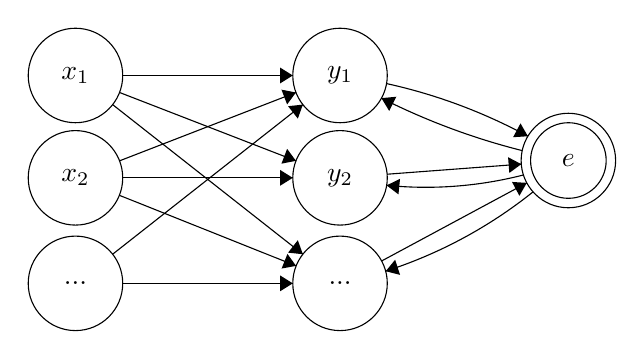
\begin{tikzpicture}[scale=0.2]
		\tikzstyle{every node}+=[inner sep=0pt]
		\draw [black] (40.1,-42.4) circle (3);
		\draw (40.1,-42.4) node {$e$};
		\draw [black] (40.1,-42.4) circle (2.4);
		\draw [black] (25.6,-37) circle (3);
		\draw (25.6,-37) node {$y_1$};
		\draw [black] (25.6,-43.5) circle (3);
		\draw (25.6,-43.5) node {$y_2$};
		\draw [black] (25.6,-50.2) circle (3);
		\draw (25.6,-50.2) node {$...$};
		\draw [black] (8.8,-37) circle (3);
		\draw (8.8,-37) node {$x_1$};
		\draw [black] (8.8,-43.5) circle (3);
		\draw (8.8,-43.5) node {$x_2$};
		\draw [black] (8.8,-50.2) circle (3);
		\draw (8.8,-50.2) node {$...$};
		\draw [black] (37.168,-41.77) arc (-104.11092:-116.74113:43.351);
		\fill [black] (28.23,-38.44) -- (28.72,-39.25) -- (29.17,-38.35);
		\draw [black] (37.246,-43.318) arc (-75.60821:-95.71526:24.95);
		\fill [black] (28.56,-43.98) -- (29.31,-44.55) -- (29.41,-43.56);
		\draw [black] (37.857,-44.391) arc (-51.32615:-72.11948:29.448);
		\fill [black] (28.5,-49.43) -- (29.41,-49.66) -- (29.1,-48.7);
		\draw [black] (11.8,-37) -- (22.6,-37);
		\fill [black] (22.6,-37) -- (21.8,-36.5) -- (21.8,-37.5);
		\draw [black] (11.6,-42.42) -- (22.8,-38.08);
		\fill [black] (22.8,-38.08) -- (21.88,-37.9) -- (22.24,-38.84);
		\draw [black] (11.16,-48.35) -- (23.24,-38.85);
		\fill [black] (23.24,-38.85) -- (22.3,-38.95) -- (22.92,-39.74);
		\draw [black] (11.6,-38.08) -- (22.8,-42.42);
		\fill [black] (22.8,-42.42) -- (22.24,-41.66) -- (21.88,-42.6);
		\draw [black] (11.16,-38.85) -- (23.24,-48.35);
		\fill [black] (23.24,-48.35) -- (22.92,-47.46) -- (22.3,-48.25);
		\draw [black] (11.8,-43.5) -- (22.6,-43.5);
		\fill [black] (22.6,-43.5) -- (21.8,-43) -- (21.8,-44);
		\draw [black] (11.8,-50.2) -- (22.6,-50.2);
		\fill [black] (22.6,-50.2) -- (21.8,-49.7) -- (21.8,-50.7);
		\draw [black] (11.59,-44.61) -- (22.81,-49.09);
		\fill [black] (22.81,-49.09) -- (22.26,-48.33) -- (21.89,-49.26);
		\draw [black] (28.555,-37.515) arc (77.60625:61.5417:34.266);
		\fill [black] (37.53,-40.86) -- (37.06,-40.04) -- (36.59,-40.92);
		\draw [black] (28.59,-43.27) -- (37.11,-42.63);
		\fill [black] (37.11,-42.63) -- (36.27,-42.19) -- (36.35,-43.19);
		\draw [black] (28.24,-48.78) -- (37.46,-43.82);
		\fill [black] (37.46,-43.82) -- (36.52,-43.76) -- (36.99,-44.64);
	\end{tikzpicture}
	\caption{An example of graphical model for exclusive coincidence classes. }
	\label{fig:ecc_graphical_models}
\end{figure}
The  $e$ node with double line represents an inhibitory neuron. All $y$ nodes are connected to it, meaning that they are mutually exclusive and only one of them can become active at the same time. All the excitatory $x$ nodes connected to any particular $y$ will contribute to its activation. The example above represents a bipartite graph, making it look like a feedforward network but in the more general case the directed connections could go both ways. The model does not need to be arranged in layers either.  

ECC are not trained using backpropagation. It is not even possible for two reasons. First is that binary values are not differentiable and second is that $\boldsymbol{y}$ are dependent on one another. Hebbian learning is necessary, but it is not sufficient. 

Suppose that observation $\boldsymbol{x}$ produces certain vector of evidence $\boldsymbol{s}=\boldsymbol{x}W$. The winning explanation $y_k=1$ is then selected using $k=argmax_j s_j$. The remaining explanations are inactive $y_j=0$ for all other $j\ne k$.
The hebbian learning tells us to strengthen $w_{ji}$ for all $i$ such that $x_i$ is active. Neurons in ECC networks work like coincidence detectors and their goal is to build stronger connections with those inputs that often occur together. The update rule is as follows
\[
w_{ik} := w_{ik} + \epsilon \text{ if } x_i=1
\]
where $\epsilon$ is some small learning rate that defines plasticity of the neuron. Different neurons could potentially use distinct $\epsilon$ values. In the real brain this is often affected by hormones. 

The hebbian rule above can only increment the weights. In order to prevent them from becoming too large, we follow this update by a normalization step.
\[
w_{ik} := \frac{w_{ik}}{ \sum_{ï} w_{ïk}} 
\]
The weights within a column must sum up to $1$. As a result, the connections $w_{ik}$ that rarely drive activity of $y_k$ will gradually vanish. In the real brain, neurons cannot grow their dendrites indefinitely. Physical limits prevent them from making too many connections. Building a synapse to new input may come at the cost of losing other, less useful ones. Similarly, there is a limit to the neuron's activity. An individual neuron cannot fire all the time. We implement this limitation using the vector $\boldsymbol{a}$. Each neuron $y_j$ has a corresponding activity value $a_j$.
When $y_j$ fires, we decrement $a_j$ by a constant factor.
\[
a_j := a_j - \alpha \text{ if } y_j \text{ fired}
\]
Now we can include $\boldsymbol{a}$ in the computation of $k$.
\[\boldsymbol{s} = \boldsymbol{x}W \]
\[\boldsymbol{r} = \boldsymbol{s} + \boldsymbol{a} \]
\[k = \argmax_j r_j \]

All of the mechanisms presented so far are necessary. Without weight normalisation, the values would run off into infinity. The activity vector $\boldsymbol{a}$ allows for entropy maximisation. It ensures that all explanations
$\boldsymbol{y}$ self-organise in an optimal way. No $y$ should be able to dominate all others. Without $\boldsymbol{a}$, the network would produce trivial explanations by routing all activity to a single $y$ and leaving all others idle. By maximising entropy, we ensure that every $y$ carries plenty of information, that could be useful in higher layers.

The final algorithm looks as follows
\begin{lstlisting}
def infer(x,W,a,learning_enabled):
    s = x * W
    r = s + a
    k = argmax(r)
    if s[k] <= threshold:
        pass    // filter-out noise (optional)
    if learning_enabled:
        a[k] -= alpha
        W[:, k] += x * plasticity_constant[k]
        W[:, k] /= sum(W[:, k])
        // the W[:, k] notation stands for 
        // k-th column of a matrix
    return k
\end{lstlisting}

\iffalse
If we tried to use it on any data we would see that it struggles with building  any meaningful representations of data. Adding more layers would only lead to even worse performance. The problem is that ECC use two types of layers. What we have so far is only the ``convergent'' layer, but training will not work without adding ``separation'' layer. Consider the problem of modelling $\boldsymbol{x}\in\{[1,1,0],[0,1,1]\}$. We would like to assign these two vectors to different $y_1$ and $y_2$. A convergent layer will always try to generalise common information and it will notice that the two vectors share $\frac{1}{3}$ of their bits in common. As a result the layer will produce two almost identical weight vectors for both $y_1$ and $y_2$. Entropy maximisation will then cause the network to oscillate between the two explanations at random. To address this issue we need some mechanism to represent logical negations of features like $x_1\wedge \neg x_3$ and $\neg x_1\wedge x_3$. Such mechanism is called the pattern separation. 



In figure \ref{fig:ecc_graphical_models} every node $y$ sends input to the same $e$ and then $e$ inhibits all $y$. As a result all $y$ regulate themselves and each other. It is possible to build a graph like in figure \ref{fig:ecc_sep_graphical_models}, where these connections are not symmetric.
\begin{figure}[!htbp]
	\centering
	
	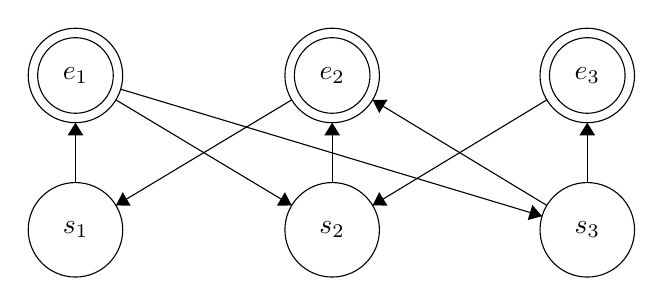
\begin{tikzpicture}[scale=0.2]
		
		\tikzstyle{every node}+=[inner sep=0pt]
		\draw [black] (7.2,-40.4) circle (3);
		\draw (7.2,-40.4) node {$e_1$};
		\draw [black] (7.2,-40.4) circle (2.4);
		\draw [black] (7.2,-50.2) circle (3);
		\draw (7.2,-50.2) node {$s_1$};
		\draw [black] (23.5,-50.2) circle (3);
		\draw (23.5,-50.2) node {$s_2$};
		\draw [black] (39.7,-50.2) circle (3);
		\draw (39.7,-50.2) node {$s_3$};
		\draw [black] (23.5,-40.4) circle (3);
		\draw (23.5,-40.4) node {$e_2$};
		\draw [black] (23.5,-40.4) circle (2.4);
		\draw [black] (39.7,-40.4) circle (3);
		\draw (39.7,-40.4) node {$e_3$};
		\draw [black] (39.7,-40.4) circle (2.4);
		\draw [black] (9.77,-41.95) -- (20.93,-48.65);
		\fill [black] (20.93,-48.65) -- (20.5,-47.81) -- (19.99,-48.67);
		\draw [black] (10.07,-41.27) -- (36.83,-49.33);
		\fill [black] (36.83,-49.33) -- (36.21,-48.62) -- (35.92,-49.58);
		\draw [black] (7.2,-47.2) -- (7.2,-43.4);
		\fill [black] (7.2,-43.4) -- (6.7,-44.2) -- (7.7,-44.2);
		\draw [black] (23.5,-47.2) -- (23.5,-43.4);
		\fill [black] (23.5,-43.4) -- (23,-44.2) -- (24,-44.2);
		\draw [black] (20.93,-41.95) -- (9.77,-48.65);
		\fill [black] (9.77,-48.65) -- (10.71,-48.67) -- (10.2,-47.81);
		\draw [black] (39.7,-47.2) -- (39.7,-43.4);
		\fill [black] (39.7,-43.4) -- (39.2,-44.2) -- (40.2,-44.2);
		\draw [black] (37.13,-48.65) -- (26.07,-41.95);
		\fill [black] (26.07,-41.95) -- (26.49,-42.79) -- (27.01,-41.94);
		\draw [black] (37.13,-41.95) -- (26.07,-48.65);
		\fill [black] (26.07,-48.65) -- (27.01,-48.66) -- (26.49,-47.81);
	\end{tikzpicture}
	\caption{Exclusive coincidence classes with asymmetric inhibition.}
	\label{fig:ecc_sep_graphical_models}
\end{figure}
 One excitatory neuron could drive inhibition of other excitatory neurons but not itself. Such a configuration allows the network to represent more sophisticated interactions between features, like $s_1\wedge\neg s_2 \wedge \neg s_3$,  $\neg s_1 \wedge s_2$ or $s_3\wedge\neg s_1 \wedge s_2$.  
 
Suppose that observations $\boldsymbol{x}$ are vectors of $n$ bits. In order to represent all possible conjunctions of negated and non-negated bits we would need to map $\boldsymbol{s}$ onto $2^n$ neurons in $\boldsymbol{y}$ layer. As we use sparse population coding,  we know that only a small fraction of bits in $\boldsymbol{x}$ will be active at any given time. Hence in practice it suffices to only use $\boldsymbol{y}$ of length $2n$ or a little less. We also do not need to keep individual inhibitory neurons in the memory. As the number of neurons increases, the effects of inhibition become approximately equivalent to choosing top $k$ highest activations. This $k$ is analogical to the top 1 best explanation in convergent layer. We will use bold $\boldsymbol{k}$ to denote a vector top $k$ elements $\boldsymbol{k}=[k_1,k2,...k_k]$ used in separation layer. 
The weights $W$ are sparse and initialised randomly. They do not need to be trained, because we do not intend to detect any coincidences (the plasticity $\epsilon$ is $0$). 
\fi

\section{Fundamental theory}

Learning the joint probability $p(\boldsymbol{x})$ is a daunting task. Bayesian models, belief nets and deep neural networks build some graphical model and then factor out this distribution as
\[
p(\boldsymbol{x})=\prod_{y} p(\boldsymbol{y}|\pi(y))
\]
where $\pi(y)$ denotes parent/neighbours of $y$ in the graph. ECC networks take a different approach: 
\[
p(\boldsymbol{x})=\sum_{j} p(\boldsymbol{x},y_j)
\]
We could say that the two are ``orthogonal'' to each other in the sense that one is a multiplicative and the other is an additive factorization of $p(\boldsymbol{x})$.  While Bayesian and variational inference rely on independence of certain nodes $p(\boldsymbol{x})=p(x_1|\boldsymbol{y})p(x_2|\boldsymbol{y})...p(x_n|\boldsymbol{y})$, ECC try to partition $p(\boldsymbol{x})$ into mutually exclusive ``coincidence classes''
$p(\boldsymbol{x})=p(\boldsymbol{x},y_1)+p(\boldsymbol{x},y_2)+...+p(\boldsymbol{x},y_m)$. It could be seen as a linear combination of joint probability distributions
\[
p(\boldsymbol{x})=\sum_{j} p(\boldsymbol{x}|y_j) p(y_j)
\]
where $p(\boldsymbol{x}|y_j)$ are vectors and $p(y_j)$ are scalars with the constraint that all  $p(y_j)$ sum up to one $\sum_{j} p(y_j)=1$. The conditional probability $p(\boldsymbol{x}|y_j)$  is not modelled directly. Instead, it is possible to turn an ECC network ``upside-down'' and use it as a generative model. 
\begin{lstlisting}
def generate(c, W, j):
    x = [0, 0, ... , 0] // n zeroes
    repeat c times:
        i = random(W[:, j])
        x[i] = 1
    return x
\end{lstlisting}
The \texttt{random} function chooses a number between $1$ and $n$ according to distribution provided by $W_j$ ($j^{th}$ column of $W$). The \texttt{generate} function can be used to produce observation $\boldsymbol{x}$ with cardinality $\lVert\boldsymbol{x} \rVert^2=\boldsymbol{x}\boldsymbol{x}^{T}$ (number of ones) less than or equal to $c$.  The probability of generating $\boldsymbol{x}$ in exactly $c=\lVert\boldsymbol{x} \rVert^2$ steps is given by 
 \[
 p(\boldsymbol{x}|y_j, \lVert\boldsymbol{x} \rVert^2 = c) = \frac{c!}{n^c}\prod_{x_i\in\boldsymbol{x}} w_{ij}
 \]
The weights represent probability $w_{ij} = p(x_i \in \boldsymbol{x}| y_j)$, which is not to be confused with $p(x_i|y_j)=\mathbb{E}(x_i|y_j)$. Instead $p(x_i \in \boldsymbol{x}| y_j)$ is defined as
\begin{gather*}
\sum_{i=1}^{n} p(x_i \in \boldsymbol{x}| y_j) = 1 \\
p(x_i \in \boldsymbol{x}| y_j) =
\frac{\sum_{\boldsymbol{x}\in\{0,1\}^n}x_i  p(\boldsymbol{x}|y_j) }{\sum_{ï=1}^{n} \sum_{\boldsymbol{x}\in\{0,1\}^n}    x_{ï}  p(\boldsymbol{x}|y_j) } = \frac{\mathbb{E}(x_i|y_j)}{\sum_{ï=1}^{n} \mathbb{E}(x_{ï}|y_j)} =  \frac{p(x_i|y_j)}{\sum_{ï=1}^{n} p(x_{ï}|y_j)} 
\end{gather*}
Therefore
\[
W_j = \frac{1}{d}\mathbb{E}(\boldsymbol{x}|y_j), \text{ where }d=\mathbb{E}(\boldsymbol{x}|y_j)\boldsymbol{1}^{T} 
\]
 the column $W_j$ is a normalised expectation. It should not be confused with the probability $p(\boldsymbol{x}|y_j)$
 \begin{gather*} 
p(\boldsymbol{x}|y_j) = p(\boldsymbol{x}|y_j,c<\infty) = \sum_{c=0}^{\infty} p(c) p(\boldsymbol{x}|y_j,c)
 \end{gather*}
where $p(\boldsymbol{x}|y_j,c)$ term has the following form
\[
p(\boldsymbol{x}|y_j,c) = N(\lVert\boldsymbol{x} \rVert^2 ,y_j,c)\big(\sum_{x_i\in\boldsymbol{x}} w_{ij}\big)^{ c - \lVert\boldsymbol{x} \rVert^2  }\prod_{x_i\in\boldsymbol{x}} w_{ij}
\]
where $N(\lVert\boldsymbol{x} \rVert^2 ,y_j,c)$ is some combinatorial coefficient that depends only on cardinality of $\boldsymbol{x}$ but not its contents. The inner product  $\boldsymbol{x}W_j$ gives us the probability of choosing any bit from $\boldsymbol{x}$
\[
\boldsymbol{x}W_j = \sum_{x_i\in\boldsymbol{x}} w_{ij}
\]
Let $\boldsymbol{x}_1, \boldsymbol{x}_2$ be two binary vectors, then $\boldsymbol{x}_1 \subset \boldsymbol{x}_2$ holds if $x_i\in\boldsymbol{x}_1$ implies $x_i\in\boldsymbol{x}_2$. The probability of generating a subset of $\boldsymbol{x}_2$ is given by
\[
p(\boldsymbol{x}_1 \subset \boldsymbol{x}_2|y_j,c) = (\boldsymbol{x}_2W_j)^c
\]
Let $\alpha$ be the probability of halting the generation process. Then 
\begin{gather*}
p(\boldsymbol{x}_1 \subset \boldsymbol{x}_2|y_j,c<\infty) = \alpha + (1-\alpha)\boldsymbol{x}_2W_j p(\boldsymbol{x}_1 \subset \boldsymbol{x}_2|y_j,c<\infty) \\
p(\boldsymbol{x}_1 \subset \boldsymbol{x}_2|y_j,c<\infty)(1-(1-\alpha)\boldsymbol{x}_2W_j ) = \alpha \\
p(\boldsymbol{x}_1 \subset \boldsymbol{x}_2|y_j,c<\infty) = \frac{\alpha}{1-(1-\alpha)\boldsymbol{x}_2W_j } \\
\end{gather*}

\section{Universal approximation}

ECC networks can approximate any $p(\boldsymbol{x})$ with only two layers. The first layer contains $2^n$ hidden neurons $\boldsymbol{y}$, one for every possible binary vector $\{0,1\}^n$. For every $\boldsymbol{x} \in \{0,1\}^n$, there exists $y_j$ such that the weights $W_j$ are uniformly distributed for all $x_i \in \boldsymbol{x}$ and zero everywhere else. The second layer $\boldsymbol{z}$ takes input from $\boldsymbol{y}$ and produces a single output $\boldsymbol{z}=[z_1]$. For every $y_j$ there exists a single weight to $z_1$ whose value determines the probability $p(y_j)$. 
 
The probability $p(\boldsymbol{x})$ will be correctly approximated if we can show that the ECC network generates samples using the same distribution. The \texttt{generate} function expects $j$ as one of its parameters. We can choose it using the second layer and then run \texttt{generate(c,W,j)} for some sufficiently large number $c=\infty$. This will almost surely result in producing  $\boldsymbol{x}$ such that $x_i\in \boldsymbol{x}$ for all $W_{ij}>0$. End of proof. 

There are several important remarks to be made. Modelling $p(\boldsymbol{x})$ using $2^n$ hidden neurons is not efficient. By introducing another layer $\boldsymbol{z}$ we could approximate one $z_h$ using a combination of  simpler ones from an intermediate layer $\boldsymbol{y}$.
\[
p(\boldsymbol{x}|z_h) = \sum_{j} p(y_j|z_h) p(\boldsymbol{x}|y_j)
\] 
The probability $p(y_j|z_h)$ is not represented directly. The weights of connections between $\boldsymbol{y}$ and $\boldsymbol{z}$ only encode the probability $p(y_j\in \boldsymbol{y}|z_h)$, which is defined analogically as before. 

The \texttt{generate} function can be generalised to much deeper multi-layer architectures as follows
\begin{lstlisting}
// W_array contains W matrices of consecutive layers.
// The order is reverse (deepest layer comes first)
def generate_deep(c, W_array, j):
    x = [0, 0, ... , 0] // n zeroes
    repeat c times:
        i = j
        for W in W_array
            i = random(W[:, i])
        x[i] = 1
    return x
\end{lstlisting}
This procedure will iteratively propagate the activation from top to bottom. It models the following expectation
\[
p(x_i\in \boldsymbol{x}|z_h) = \sum_{j} p(y_j|z_h) p(x_i \in \boldsymbol{x}|y_j)
\]
\[
\mathbb{E}(\boldsymbol{x}|z_h) = \sum_{j} p(y_j\in \boldsymbol{y}|z_h) \mathbb{E}(\boldsymbol{x}|y_j)
\] 

The key observation here is that the $j$ argument is still necessary. This means that the user still needs to somehow decide which hidden neuron to sample.

 




\section{Linear probability spaces and eigendistributions}

ECC networks learn by decomposing the probability $p(\boldsymbol{x})$ into its ``principal components''.   In the general case consider  $\mathcal{P} \subset \mathcal{X} \rightarrow [0,1]$ to be some set of distributions where $\mathcal{X}$ is the set of observations $\boldsymbol{x}$. The conditional distribution $p(\boldsymbol{x},y_j)$ must be an element of $\mathcal{P}$. The marginal distribution $p(\boldsymbol{x})$ is a member of probability space generated by $\mathcal{P}$ if it can be represented as a linear combination of its elements.


The ECC networks attempt to approximate $p(\boldsymbol{x}|y_j)$  using the matrix $W$. The challenge here lies in the fact that such eigendecomposition of joint distributions is an ill-defined problem. There might exist infinitely many coefficients (summed under Lebesgue integral)
\[
p(\boldsymbol{x})= \int_y p(\boldsymbol{x}|y) p(y)
\]
Most of those coefficients would be very small. We are hoping to approximate $p(\boldsymbol{x})$ with only a finite number of them. We could draw an analogy to data compression algorithms, where we try to ``compress'' $p(\boldsymbol{x})$ by only keeping the $m$ largest eigenvalues and truncating all the rest. The only difference here is that the probabilities must sum up to one and if we truncated any of the eigendistributions,  this would be violated. Instead we can reduce the number of used eigendistributions by adding some of them together. 
\[
p(\boldsymbol{x}|y_1) p(y_1)+p(\boldsymbol{x}|y_2) p(y_2) = 
p(\boldsymbol{x}|y_1\text{ or }y_2) (p(y_1)+p(y_2))
\]
If we could know $p(\boldsymbol{x}|y_1\text{ or }y_2)$ exactly, then we would be able to find the exact solution to 
\[
\int_y p(\boldsymbol{x}|y) p(y) = p(\boldsymbol{x}| y_1\text{ or }y_2 \text{ or }...)\int_y p(y)= p(\boldsymbol{x}) \cdot 1
\]
and the problem of modelling $p(\boldsymbol{x})$ would become trivial. The task becomes more interesting when we can't represent  $p(\boldsymbol{x}|y_1\text{ or }y_2)$ directly. For example, our implementation of ECC networks represents $p(\boldsymbol{x}|y)$ using a weight matrix $W$, which implies mutual independence of all $x$ variables
\[
p(\boldsymbol{x}|y_j) = p(x_1|y_j)p(x_2|y_j)...p(x_n|y_j) = \boldsymbol{x} W_j
\]
We can only approximate $p(\boldsymbol{x}|y_1\text{ or }y_2)$
using the combination
\[
p(\boldsymbol{x}|y_1\text{ or }y_2) p(y_1\text{ or }y_2)= p(\boldsymbol{x}|y_1) p(y_1)+p(\boldsymbol{x}|y_2) p(y_2) \approx \boldsymbol{x}W_1p(y_1) + \boldsymbol{x}W_2 p(y_2)
\]
under the assumption that $p(y_2)$ is a much smaller eigenvalue than $p(y_1)$.
The above approximation would be an exact equality only in a special case, where the two eigendistributions are linearly dependent (equal up to some constant $c$):
\[p(\boldsymbol{x},y_2)=c p(\boldsymbol{x},y_1)\]
In practice it is unlikely that we could find such equalities, but the more similar the two summed distributions are, the more precise our approximation of $p(\boldsymbol{x}|y_1\text{ or }y_2)$ would be. 

Learning is the matter of clustering the eigendistributions by their similarity and then summing up all the elements within the same cluster to obtain the final approximation. If we have only a finite number of observations $\boldsymbol{x}$, then we can find an optimal solution to this problem by brute-force. Alternatively a more efficient approach, might be to use modified k-means algorithm, which always converges to a local optimum. 

\section{Convergence proof}

Let us treat $W_j$ as points in space $\mathbb{R}^n$. Let $\{0,1\}^n$  be the set of observations. Every $\boldsymbol{x}\in \{0,1\}^n$ has some probability $p(\boldsymbol{x})$ and all the other points in $\mathbb{R}^n$ have probability $0$. We may not know the exact $p(\boldsymbol{x})$ but we can approximate it using empirical distribution. Define $C(y_j)$ as the cluster of all the $\boldsymbol{x}$ such that
\[
 C(y_j) = \{\boldsymbol{x} :  j = \argmax(\boldsymbol{x} W) \} 
\]
In other words, $\boldsymbol{x}$ will be assigned to the cluster $C$ of this  $y_j$, which has the highest cosine similarity $\boldsymbol{x}W_j$. (Side note: while in the ``standard'' k-means algorithm, the distance metric between points is euclidean, here we use angular distance. Moreover all the observations $\boldsymbol{x}$ should have approximately the same number of $1$'s so their euclidean norms should be similar and as a result all $\boldsymbol{x}$ will approximately lie on a sphere.  Hence we are working on a $S^n$ manifold embedded in $\mathbb{R}^n$ space.)  The mean $\mu(y_j)$ of cluster is given by 
\begin{gather*}
	\mathbb{E}(\boldsymbol{x}|y_j) = \frac{\sum_{\boldsymbol{x}\in C(y_j)} \boldsymbol{x}p(\boldsymbol{x})}{\sum_{\boldsymbol{x}\in C(y_j)} p(\boldsymbol{x})} = \frac{\sum_{\boldsymbol{x}\in C(y_j)} \boldsymbol{x}p(\boldsymbol{x})}{p(y_j)} \\
	\mu(y_j)  = \frac{\mathbb{E}(\boldsymbol{x}|y_j)}{\sum_{ï=1}^{n}\mathbb{E}(x_{ï}|y_j)}
\end{gather*}
K-means clustering works by iteratively recomputing $C(y_j)^{(t)}$ at time-step $t$ for all $j$ and then assigning $\mu(y_j)^{(t)}$ to be the new value of $W_j^{(t+1)}$ at the next time-step. Let the loss function be

\[
\mathcal{L} = \sum_{j=1}^{m} \sum_{\boldsymbol{x}\in C(y_j)} \lVert  W_j - \boldsymbol{x}\rVert^1p(\boldsymbol{x})
\]
where $\lVert \cdot \rVert^1$ stands for $l_1$ metric (Manhattan distance). We can prove that $\mathcal{L}$ always decreases and is bounded (can't be negative), hence the learning converges. First we show that
\[
\mathcal{L}(s_k)^{(t)} =\sum_{j=1}^{m} \sum_{\boldsymbol{x}\in C(y_j)^{(t)}} \lVert  W_j^{(t)} - \boldsymbol{x}\rVert^1p(\boldsymbol{x})
\ge \sum_{j=1}^{m} \sum_{\boldsymbol{x}\in C^{(t)}(y_j)} \lVert  W_j^{(t+1)} - \boldsymbol{x}\rVert^1p(\boldsymbol{x})
\]
and then
\[
\sum_{j} \sum_{\boldsymbol{x}\in C(y_j)^{(t)}} \lVert W_j^{(t+1)} - \boldsymbol{x}\rVert^1 p(\boldsymbol{x}) \ge \sum_{j} \sum_{\boldsymbol{x}\in C(y_j)^{(t+1)}} \lVert W_j^{(t+1)}-\boldsymbol{x}\rVert^1 p(\boldsymbol{x}) = \mathcal{L}^{(t+1)}
\]
The first inequality follows from the definition of $W_j^{(t+1)} = \mu(y_j)^{(t)}$, which is a form of maximum likelihood estimation.
\[
\sum_{j=1}^{m} \sum_{\boldsymbol{x}\in C(y_j)^{(t)}} \lVert  W_j^{(t)} - \boldsymbol{x}\rVert^1p(\boldsymbol{x})
\ge \sum_{j=1}^{m} \sum_{\boldsymbol{x}\in C^{(t)}(y_j)} \lVert  \mu(y_j)^{(t)} - \boldsymbol{x}\rVert^1p(\boldsymbol{x})
\]
The second inequality follows from the fact that $C(y_j)^{(t)}$ will differ from $C(y_j)^{(t+1)}$ only if there exists some $\boldsymbol{x} \in C(y_j)^{(t)}$ such that we could find some different $y_h$ with the property $\boldsymbol{x} W_k \ge \boldsymbol{x} W_j$. Then such $\boldsymbol{x}$ would be moved from $C(y_j)^{(t)}$ to $C(y_h)^{(t+1)}$, but this could only result in the $\mathcal{L}^{(t+1)}$ to increase (or stay constant), because 
\begin{gather*}
	\boldsymbol{x} W_h \ge \boldsymbol{x} W_j \\
	\sum_{x_i\in\boldsymbol{x} }w_{ih} \ge \sum_{x_i\in\boldsymbol{x} }w_{ij} \\
	\sum_{x_i\in\boldsymbol{x} }1-w_{ih} \le \sum_{x_i\in\boldsymbol{x} }1-w_{ij} \\
	\sum_{x_i\in\boldsymbol{x} }\vert 1-w_{ih}\vert^1 \le \sum_{x_i\in\boldsymbol{x} }\vert 1-w_{ij}\vert^1
\end{gather*}
Let $1-\boldsymbol{x}$ be the complement of binary vector (ones and zeroes flipped). Because weights sum up to $1$, this implies that
\begin{gather*}
(1-\boldsymbol{x}) W_h \le (1-\boldsymbol{x}) W_j \\
\sum_{x_i\notin\boldsymbol{x} }w_{ih} \le \sum_{x_i\notin\boldsymbol{x} }w_{ij} \\
\sum_{x_i\notin\boldsymbol{x} }\vert 0-w_{ih}\vert^1 \le \sum_{x_i\notin\boldsymbol{x} }\vert 0-w_{ij}\vert^1
\end{gather*}
Adding the two inequalities together by sides we obtain
\[
	\lVert \boldsymbol{x} - W_h \rVert^1 \le \lVert  \boldsymbol{x} - W_j \rVert^1
\]
This concludes the proof.

So far we have shown that learning converges without accounting for $\boldsymbol{a}$ and entropy maximisation. To address this, let us we modify the definition of $C(y_j)$ to include $\boldsymbol{a}$ 
\[
\boldsymbol{x} \in C(y_j) \iff  j = \argmax(\boldsymbol{x} W + \boldsymbol{a})
\]
The absolute value of $\boldsymbol{a}$ does not matter, because adding a constant scalar does not change result of $argmax$ function  
\[
\argmax(\boldsymbol{x} W + \boldsymbol{a} + c)  = \argmax(\boldsymbol{x} W + \boldsymbol{a} )
\]
We also know that $0 \le \boldsymbol{x} W_j \le 1$, which implies that $max(\boldsymbol{a})-min(\boldsymbol{a})\le 1$ because otherwise the maximum element of $\boldsymbol{a}$ would entirely dominate all others and increasing $max(\boldsymbol{a})$ beyond $min(\boldsymbol{a})+1$ would not make any difference. Therefore without loss of generality we can assume that $max(\boldsymbol{a})=0$ and $min(\boldsymbol{a})\ge -1$.

Under such assumption, we can now change the loss function. Instead of $-\mathbb{E}(s_k)$, we will use 
$-\mathbb{E}(s_k+a_k)$, defined as
\[
\mathbb{E}(s_k+a_k) = \sum_{j=1}^{m} \sum_{\boldsymbol{x}\in C(y_j)} (\boldsymbol{x}W_j +a_j)p(\boldsymbol{x})
\]
The vector $\boldsymbol{a}$ functions as a regularization term. Most of the previous convergence proof will still hold, with only minor changes. In many cases, the $a_j$ term can be factored out of the summation and then cancelled out on both sides of inequality. 



\section{Convolutional networks}

In this section we introduce the final working model of a network that can build meaningful receptive fields $p(\boldsymbol{x}|y_j)$. In general case the topology of an ECC network might be chaotic and highly recurrent. We distinguish a special subset of topologies that are arranged in a form of multi-layer convolutional networks. Figure \ref{fig:ecc_conv_machine} shows an example of a single convolutional layer. Several of them could be stacked to form a multi-layer network. 

\begin{figure}[!htbp]
	\centering

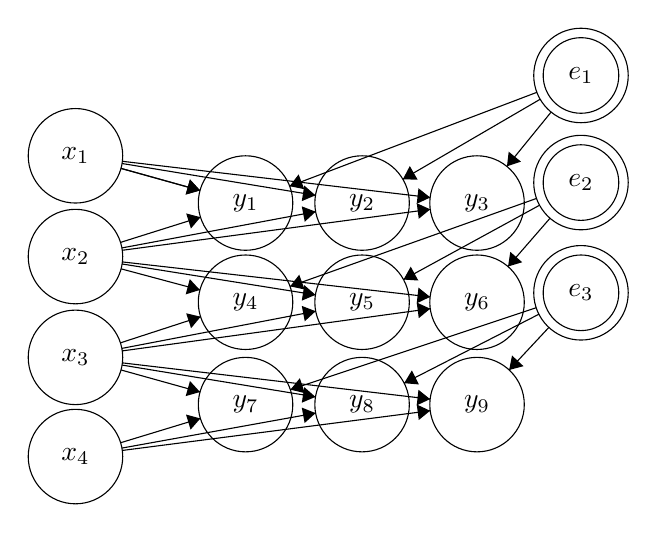
\begin{tikzpicture}[scale=0.2]
	\tikzstyle{every node}+=[inner sep=0pt]
	\draw [black] (8,-12.4) circle (3);
	\draw (8,-12.4) node {$x_1$};
	\draw [black] (8,-18.8) circle (3);
	\draw (8,-18.8) node {$x_2$};
	\draw [black] (8,-25.2) circle (3);
	\draw (8,-25.2) node {$x_3$};
	\draw [black] (8,-31.5) circle (3);
	\draw (8,-31.5) node {$x_4$};
	\draw [black] (18.8,-15.4) circle (3);
	\draw (18.8,-15.4) node {$y_1$};
	\draw [black] (33.5,-15.4) circle (3);
	\draw (33.5,-15.4) node {$y_3$};
	\draw [black] (26.2,-15.4) circle (3);
	\draw (26.2,-15.4) node {$y_2$};
	\draw [black] (18.8,-21.7) circle (3);
	\draw (18.8,-21.7) node {$y_4$};
	\draw [black] (26.2,-21.7) circle (3);
	\draw (26.2,-21.7) node {$y_5$};
	\draw [black] (33.5,-21.7) circle (3);
	\draw (33.5,-21.7) node {$y_6$};
	\draw [black] (18.8,-28.2) circle (3);
	\draw (18.8,-28.2) node {$y_7$};
	\draw [black] (26.2,-28.2) circle (3);
	\draw (26.2,-28.2) node {$y_8$};
	\draw [black] (33.5,-28.2) circle (3);
	\draw (33.5,-28.2) node {$y_9$};
	\draw [black] (40.1,-7.3) circle (3);
	\draw (40.1,-7.3) node {$e_1$};
	\draw [black] (40.1,-7.3) circle (2.4);
	\draw [black] (40.1,-14.1) circle (3);
	\draw (40.1,-14.1) node {$e_2$};
	\draw [black] (40.1,-14.1) circle (2.4);
	\draw [black] (40.1,-21.1) circle (3);
	\draw (40.1,-21.1) node {$e_3$};
	\draw [black] (40.1,-21.1) circle (2.4);
	\draw [black] (10.89,-13.2) -- (15.91,-14.6);
	\fill [black] (15.91,-14.6) -- (15.27,-13.9) -- (15,-14.86);
	\draw [black] (10.86,-17.9) -- (15.94,-16.3);
	\fill [black] (15.94,-16.3) -- (15.03,-16.06) -- (15.33,-17.02);
	\draw [black] (10.89,-13.2) -- (15.91,-14.6);
	\fill [black] (15.91,-14.6) -- (15.27,-13.9) -- (15,-14.86);
	\draw [black] (10.96,-12.89) -- (23.24,-14.91);
	\fill [black] (23.24,-14.91) -- (22.53,-14.29) -- (22.37,-15.28);
	\draw [black] (10.95,-18.25) -- (23.25,-15.95);
	\fill [black] (23.25,-15.95) -- (22.37,-15.61) -- (22.56,-16.59);
	\draw [black] (10.98,-12.75) -- (30.52,-15.05);
	\fill [black] (30.52,-15.05) -- (29.78,-14.46) -- (29.67,-15.45);
	\draw [black] (10.97,-18.4) -- (30.53,-15.8);
	\fill [black] (30.53,-15.8) -- (29.67,-15.41) -- (29.8,-16.4);
	\draw [black] (37.3,-8.37) -- (21.6,-14.33);
	\fill [black] (21.6,-14.33) -- (22.53,-14.52) -- (22.17,-13.58);
	\draw [black] (37.51,-8.81) -- (28.79,-13.89);
	\fill [black] (28.79,-13.89) -- (29.73,-13.92) -- (29.23,-13.05);
	\draw [black] (38.2,-9.63) -- (35.4,-13.07);
	\fill [black] (35.4,-13.07) -- (36.29,-12.77) -- (35.51,-12.14);
	\draw [black] (37.47,-15.54) -- (28.83,-20.26);
	\fill [black] (28.83,-20.26) -- (29.77,-20.32) -- (29.29,-19.44);
	\draw [black] (38.13,-16.37) -- (35.47,-19.43);
	\fill [black] (35.47,-19.43) -- (36.37,-19.16) -- (35.61,-18.5);
	\draw [black] (37.27,-15.11) -- (21.63,-20.69);
	\fill [black] (21.63,-20.69) -- (22.55,-20.89) -- (22.21,-19.95);
	\draw [black] (38.06,-23.3) -- (35.54,-26);
	\fill [black] (35.54,-26) -- (36.45,-25.76) -- (35.72,-25.08);
	\draw [black] (37.43,-22.46) -- (28.87,-26.84);
	\fill [black] (28.87,-26.84) -- (29.81,-26.92) -- (29.36,-26.03);
	\draw [black] (37.25,-22.05) -- (21.65,-27.25);
	\fill [black] (21.65,-27.25) -- (22.56,-27.47) -- (22.25,-26.52);
	\draw [black] (10.9,-19.58) -- (15.9,-20.92);
	\fill [black] (15.9,-20.92) -- (15.26,-20.23) -- (15,-21.2);
	\draw [black] (10.85,-24.28) -- (15.95,-22.62);
	\fill [black] (15.95,-22.62) -- (15.03,-22.4) -- (15.34,-23.35);
	\draw [black] (10.96,-19.27) -- (23.24,-21.23);
	\fill [black] (23.24,-21.23) -- (22.53,-20.61) -- (22.37,-21.6);
	\draw [black] (10.95,-24.63) -- (23.25,-22.27);
	\fill [black] (23.25,-22.27) -- (22.37,-21.93) -- (22.56,-22.91);
	\draw [black] (10.98,-19.14) -- (30.52,-21.36);
	\fill [black] (30.52,-21.36) -- (29.78,-20.77) -- (29.67,-21.77);
	\draw [black] (10.97,-24.79) -- (30.53,-22.11);
	\fill [black] (30.53,-22.11) -- (29.67,-21.72) -- (29.8,-22.71);
	\draw [black] (10.89,-26) -- (15.91,-27.4);
	\fill [black] (15.91,-27.4) -- (15.27,-26.7) -- (15,-27.66);
	\draw [black] (10.87,-30.62) -- (15.93,-29.08);
	\fill [black] (15.93,-29.08) -- (15.02,-28.83) -- (15.31,-29.79);
	\draw [black] (10.96,-25.69) -- (23.24,-27.71);
	\fill [black] (23.24,-27.71) -- (22.53,-27.09) -- (22.37,-28.08);
	\draw [black] (10.95,-30.96) -- (23.25,-28.74);
	\fill [black] (23.25,-28.74) -- (22.37,-28.39) -- (22.55,-29.37);
	\draw [black] (10.98,-25.55) -- (30.52,-27.85);
	\fill [black] (30.52,-27.85) -- (29.78,-27.26) -- (29.67,-28.25);
	\draw [black] (10.98,-31.11) -- (30.52,-28.59);
	\fill [black] (30.52,-28.59) -- (29.67,-28.19) -- (29.8,-29.18);
\end{tikzpicture}
	\caption{A single layer of exclusive coincidence machine with one-dimensional convolution. The input size is $4$ columns, each with one channel. The hidden layer has $3$ columns, each with $3$ channels. The neurons within the same column are all mutually exclusive. Every hidden column draws input from two input columns around it, meaning that in this case the kernel size is $2$. The stride is $0$. }
	\label{fig:ecc_conv_machine}
\end{figure} 

The neuron $y_1$ can ``see'' input coming from $x_1$ and $x_2$. We say that the topological receptive field $\tau$ of $y_1$ is $\tau(y_1)=\{x_1,x_2\}$. All the neurons
within the same column share common $\tau$ and compete with each other due to inhibition. Neurons across different columns have access to distinct fragments of input. As a result every column will only learn to recognise input as a specific location. 

Deep nets learn by approximating functions and the architecture of the network provides inductive priors by constraining the functions to follow certain equivariant properties. Deep convolutional networks a-priori come with the assumption of translation invariance which is enforced by sharing kernel weights. The ECC are capable of learning such equivariances on their own.

In the example from figure \ref{fig:ecc_conv_machine}, the neurons $[y_1,y_2,y_3]$ and $[y_4,y_5,y_6]$ receive inputs $[x_1,x_2]$ and $[x_2,x_3]$ respectively. If the input is indeed translation invariant then $p([x_1,x_2])=p([x_2,x_3])$ should hold by definition. In such case, hebbian learning will drive both $[y_1,y_2,y_3]$ and $[y_4,y_5,y_6]$ to develop similar factorizations
\begin{gather*}
p(\boldsymbol{x}) = p(\boldsymbol{x}|y_1)p(y_1)+  p(\boldsymbol{x}|y_2)p(y_2)+  p(\boldsymbol{x}|y_3)p(y_3)\text{ where }\boldsymbol{x}=[x_1,x_2] \\
p(\boldsymbol{x}) = p(\boldsymbol{x}|y_4)p(y_4)+  p(\boldsymbol{x}|y_5)p(y_5)+  p(\boldsymbol{x}|y_6)p(y_6)\text{ where }\boldsymbol{x}=[x_2,x_3]
\end{gather*}
such that $p(\boldsymbol{x}|y_2) \approx p(\boldsymbol{x}|y_{\sigma(4)}), p(\boldsymbol{x}|y_{3}) \approx p(\boldsymbol{x}|y_{\sigma(5)}),p(\boldsymbol{x}|y_3) \approx p(\boldsymbol{x}|y_{\sigma(6)}) $ for some permutation $\sigma$. Both columns are approximately isomorphic. We can stack multiple layers on top of each other and the equivariance will be preserved. For example let $W_1,W_2$ be the weights of connections from $[y_1,y_2,y_3]$ and   $[y_4,y_5,y_6]$ respectively, outgoing to some neuron $z_1$ in next layer. If the two columns are isomorphic then $W_1\approx\sigma W_2$. Hence it can be seen that the networks can self-organise and equivariance will emerge. The only inductive bias is the topology $\tau$. (Convolutional pattern of $\tau$ can easily emerge on its own if we assume that the neurons are embedded in a physical space and the axons are sparsely projected to some small local neighbourhood in subsequent regions of neocortex.)

This model achieves exactly what Geoffrey Hinton's capsule networks were originally meant to do. Even though $[y_1,y_2,y_3]$ and   $[y_4,y_5,y_6]$ are isomorphic, they not equivalent from information perspective. They recognise the same signal but at different locations. Deeper layers $\boldsymbol{z}$ could then access such location-carrying information and builds hierarchies of features that account for their spacial relationships. Such ECC networks can build``semantic'' models of the environment when combined with motor feedback, which will be shown in a later section.


\section{Experiments}

Convolutional ECC networks can be trained either layer-by-layer (from bottom to top) or all at once (hebbian learning works everywhere simultaneously). The only difference between the two approaches is that training layer-by-layer can be much faster and more efficient on a static dataset, whereas online learning of all layers at once allows for extracting temporal dependencies in an interactive environment. 

Network topology is determined by its sequence of convolutions. Here we present effects of all-at-once training for architecture $5\times 2 \times 20,  2\times 1 \times 54$. Figure  \ref{fig:experiment3} shows averaged receptive field $\mathbb{E}(\boldsymbol{x}|y_j)$ formed by one arbitrarily chosen column in the first hidden layer


\begin{figure}[!htbp]
	\centering
	\includegraphics[width=12cm]{predictive_coding_stacked2_experiment3 before}
	\includegraphics[width=12cm]{predictive_coding_stacked2_experiment3 after}
	\caption{Receptive fields of 20 neurons from a first hidden layer before and after training.}
	\label{fig:experiment3}
\end{figure} 

\begin{figure}[!htbp]
	\centering
	\includegraphics[width=11cm]{predictive_coding_stacked2_experiment4 before}
	\includegraphics[width=11cm]{predictive_coding_stacked2_experiment4 after}
	\caption{Receptive fields of 64 neurons in the fourth layer}
	\label{fig:experiment4}
\end{figure} 

First set of experiments Figures and \ref{fig:experiment4} represents neurons from one column in layer 3 after training.
Figure presents receptive fields of neurons from layer 4 in randomly initialised network before training and the exclusive coincidence classes that emerge after enough iterations.
At the beginning the receptive fields tend to fluctuate. Their shapes appear blurry and random. After enough iterations, the receptive fields stabilise and converge to much sharper and more detailed shapes. The training was performed by taking random 11x11 patches of MNIST images.




\section{Reinforcement learning and control}

\iffalse
The current dominant view of the brain has been heavily focused on optimisation.
All existing models of neural networks revolve around the idea that there exists some hidden error function that needs to be minimised. In reality there is nothing about the brain that resembles optimisation. Instead of fitting data, its fundamental principle is to build models of the world. In ECC networks, every single neuron tries to capture certain specific phenomenon of the external world. Every neuron is its own model. Perhaps we could summarise this idea as ``billion brains theory'', because we have billions of neurons and each one of them encodes some idea. The consciousness itself is decentralised. You can never lose your consciousness in its entirety. If your fusiform face area is damaged, you will lose the part of your consciousness that holds models of faces. If your hippocampus is removed, you will lose a fragment of consciousness that holds your recent memories.  In this view, every single neuron behaves like a miniature brain in and of itself. If $\boldsymbol{x}$ encodes the outside world, then each $y_i$ represents some tiny fragment of it. As you increase the number of neurons $\boldsymbol{y}$, you subdivide the world into billions of small interdependent ideas $p(\boldsymbol{x})=p(\boldsymbol{x},a_1)+...+p(\boldsymbol{x},a_{10^9})$.
\fi

The deep neural networks learn using backpropagation. They are inherently a supervised method of building intelligence. Even when the labels and error comes from the data itself, in a self-supervised manner, the learning still relies on the same supervised mechanisms. Deep nets can be applied to reinforcement learning problems by modelling the reward function. ECC networks on the other hand are purely unsupervised. They can't represent policy or reward function in any meaningful way. However, the biological brains are capable of performing control tasks very well. How could we achieve the same using ECC networks?


Reinforcement learning can be reformulated in a purely unsupervised way via introduction of energy $E$. The reward is defined as the derivative of energy, with respect to time
\[
R(t) = \frac{dE}{dt}
\]
When the agent finds source of energy, it will receive the feeling of reward.
Movement and action require energy. Even remaining idle will slowly lead to depletion of its reserves. This is the reason why animals tend to choose straight-line paths towards their destinations. 

The exploration and exploitation dilemma can be solved very elegantly. The energy is intrinsic to the agent. It will always know exactly how much it has and if the agent feels like it has access to abundant reserves of energy it could then decide to waste some of it by freely foraging and exploring. We can introduce a ``hunger'' constant  $h$. If $E<h$ then agent performs exploitation, otherwise it undertakes exploration.

The integral of $R$ is equivalent to sum of future rewards $R$, also commonly known as the return $G$. This is equal to the energy at some future time $E(T)$
\[
\int_{t=now}^{T} R dt = G(T) - G(now) = E(T)
\]
Suppose that sources of energy are scarce in the environment. Then finding any source of energy already has high probability of maximising the reward. Therefore we do not need to be preoccupied too much with ``maximising'' and should instead focus on ``finding'' anything at all. 

The agent never receives any reward. It doesn't actually exist. The reward is only something abstract and visible to an external observer, but internally the ECC networks have no concept of reward . This is the key difference between supervised and unsupervised reinforcement learning (figure \ref{fig:rl}). There is no reward. Instead, the network learns by modelling its effective fields. In order to define what this means, we need to assume that the agent is embodied. Let $\boldsymbol{u}$ be a binary vector representing motor neurons.
Analogically to receptive fields $p(\boldsymbol{x}|y_j)$ modelling input, the effective field
$p(\boldsymbol{u}|y_j)$ is a model of output. This is the probability that certain pattern of motor neurons activates in response to $y_j$ firing. The $\boldsymbol{y}$ neurons do not know their effective fields, hence feedback input $\boldsymbol{f}$ is necessary. It's a special type of input that carries back information about the action performed by $\boldsymbol{u}$. The receptive field $p(\boldsymbol{f}|y_j)$ works as a proxy for learning effective fields $p(\boldsymbol{u}|y_j)$. In very simple networks, both $\boldsymbol{u}$ and $\boldsymbol{f}$ might be coded using the same population of neurons, but in more complex topologies this may not be the case. Similarly we could think of $\boldsymbol{f}$ as a subpopulation of $\boldsymbol{x}$. 

The agent has two modelling tasks, both unsupervised. One of them is learning to anticipate $\boldsymbol{x}$ and $\boldsymbol{f}$ in the next time-step, knowing the current output $\boldsymbol{u}$. The second task involves planning and it tries to model the right output $\boldsymbol{u}$ that leads to the desired (distant) future internal state $E$ and $\boldsymbol{y}$. The neurons $\boldsymbol{y}$ build an internal model of the outside world and they compete for control over $\boldsymbol{u}$, similarly to how inputs $\boldsymbol{x}$ ``compete'' to trigger changes in $\boldsymbol{y}$.

\begin{figure}[!htbp]
	\centering
	\includegraphics[width=10cm]{supervised reinforcement learning}
	\includegraphics[width=10cm]{unsupervised reinforcement learning}
	\caption{Comparison of supervised (top) and unsupervised (bottom) reinforcement learning}
	\label{fig:rl}
\end{figure} 

If the agent builds an internal model of the world, that works like a map, it could then use such cognitive map to very quickly and efficiently search for energy sources. This only requires imagination, which is much cheaper than locomotion. The ECC networks do not see any reward. Instead, when the energy increases, certain neurons become temporarily more plastic than usually. This mechanism could be used to bias the cognitive map more towards places and actions that lead to the source of energy.

Once the agent has an internal map, it could then exactly know which aspects of the environment are unexplored. Unlike in the current deep reinforcement learning approaches, an agent with episodic memory would only need to visit a novel place once in order to learn about it. If the world is dynamically changing, then an attention mechanism will be necessary. If an animal sees or hears something unexpected it will focus all its attention on the novel experience. This mechanism can be explained using ECC networks as well. Suppose that the current internal model $\boldsymbol{y}$ explains all the previously experienced observations $p(\boldsymbol{x})=\sum_j p(\boldsymbol{x},y_j)$. If the agent experiences something novel that does not fit into any specific $y$, then it will be surprised. The agent will become curious and focus on the novel experience for a while. After the model  $\boldsymbol{y}$ restructures itself and learns about the new $\boldsymbol{x}$, then the agent become ``bored''. 


\section{Optimisations and efficiency benchmarks}

Sparsity enables major optimisations. We can define ECC layers with thousands of neurons, leading to $W$ matrices with millions of weights. Computing them is cheap and can be done on a single CPU because the input vector is sparse and binary. We do not need to multiply $\boldsymbol{x}W$ entirely. If we represent $\boldsymbol{x}$ as a list of indices of active neurons, then we can only iterate such list and visit only a handful of columns in $W$. The $argmax$ operation is linear. During learning we have to renormalise the winning column of $W$. This requires computing sum, which is of linear complexity. We can achieve constant complexity if we implement a stochastic algorithm, that is, we add $\epsilon$ to $w_{ik}$ for $x_i=1$ (this operation is constant because $\boldsymbol{x}$ is sparse) and then we randomly choose a few other $w_{ik}$ for $x_i=0$ and subtract $\epsilon$ from them. We might need to check if $w_{ik}>0$ in order to avoid introducing negative values. This ensures that weights always sum up to $1$.

The real brain can function on a few potatoes a day. With neuromorphic hardware, ECC networks should be able to do the same. In theory we could have human-level intelligence running on cheap small chips. It's hard to imagine what a supercomputer could achieve.

We ran benchmarks on random patches of MNIST images. Each patch was 25x25 pixels. The network had 734400 learnable parameters (and several non-learnable sparse matrices). Our implementation written in Rust was able to process 2000 images per second on a single thread on 2.7 GHz Intel i5 core. When learning was enabled, it could train on 1700 images per second.


\section{ECC are spiking networks}

The ECC can be extended to work with time series, model sequential data, detect movement and distance of objects. Let $\boldsymbol{x}^{(t)}$ and $\boldsymbol{y}^{(t)}$ be the input signal and states of neurons at time step $t$ respectively. We can concatenate several such vectors $\boldsymbol{x}^{(t-b)}\cdot \boldsymbol{x}^{(t-b+1) }\cdot ...\cdot\boldsymbol{x}^{(t)}=\boldsymbol{\hat{x}}^{(t)}$ up to $b$ steps from the past. Analogically for $\boldsymbol{\hat{y}}^{(t)}$. Now the weight matrices $W$ can span not only neurons but also their past states. The connections are now made not only across space but also time. The size of $W$ is given by $bnm$ where $n$ and $m$ is the number of input $\boldsymbol{x}$ and hidden $\boldsymbol{y}$ neurons respectively. The memory complexity is therefore cubic. There is a certain heuristic that can be exploited in order to obtain a quadratic complexity. The natural environment is time-consistent, meaning that usually $\boldsymbol{x}$ only changes a little between time steps. When the agent is idle, it may look in a specific direction for prolonged period of time and always observe the same $\boldsymbol{x}$. Therefore we could agree to only make one connection to a specific point in time per input-output pair. Hence the matrix $W$ is not a Cartesian product $[t-b,t] \times \boldsymbol{x} \times \boldsymbol{y} \rightarrow [0,1]$  but rather a function $\boldsymbol{x} \times \boldsymbol{y} \rightarrow [t-b,t] \times [t-b,t] \rightarrow [0,1]$ where $[t-b,t] \times [t-b,t]$ are the beginning and end of the time-window (relative to current time $t$).

In the case of continuous time, primitive distributions must be represented using a different data structure than a matrix. The dendrites of biological neurons carry their information at different speeds. The faster dendrites connect to recent past, whereas slower ones detect signal from to more distant past. The action potential doesn't vanish instantly. A plateau potential may linger for a certain period of time, which means that the neuronal connections can be tuned to a time-interval of some specific length. The neurons tend to fire in spike trains of specific frequency. Two subsequent spikes coming from the same input are likely correlated and do not carry additional information, hence it's pointless to have multiple connections to the same input tuned to distinct times. This again allows for reducing the complexity from cubic to quadratic. Hence the optimal data structure for representing continuous primitive distributions is a function $\boldsymbol{x} \times \boldsymbol{y} \rightarrow \mathbb{R} \times \mathbb{R} \rightarrow [0,1]$ where $\mathbb{R} \times \mathbb{R}$ represents beginning and end of time interval.

The standard ECC learning algorithm can be used to train $W$ matrices of cubic complexity. When we used the heuristic quadratic $W$, then the spike-time-dependent plasticity emerges as the optimal learning method. If the input spike comes too early, we move the time window a little to the past. If it comes too late, we move it a notch to the future. If the variance of relative spike time is high, then we stretch the time window to be longer. If the input arrives at a very predictable time, then we can narrow down the window size. 

The dendrites of biological neurons are arranged in a tree-like structure. Tuning the time-window selectivity of the dendrite will affect all of the synapses. Under such circumstances, the only way to fine-tune individual synapses is to disconnect them if the time-window of the current dendrite is unsuitable and hope that some other dendrite happens to be better tuned and could form the right synapses.	


\section{Evolving ECC networks}

The receptive fields $p(\boldsymbol{x},y_j)$ of neurons are primarily driven by their respective topologies $\tau$. We can embed the set of all neurons $\boldsymbol{y}$ in a n-dimensional euclidean space. This way we obtain a norm on all nodes in the graph. Neurons that are in close proximity, should have higher probability of developing similar topologies. Then the task of evolving ECC network becomes reduced to evolution of manifolds in a euclidean space. Kenneth Stanley's ES-HyperNEAT algorithm can be repurposed for such a task. 



\bibliographystyle{BibTeXtran}   % (uses file "BibTeXtran.bst")
\bibliography{BibTeXrefs}    







\end{document}
